\documentclass{article}
\def\ChineseVersion{1}
\usepackage{iclr2027_conference,times}
\ifdefined\ChineseVersion
  \usepackage[UTF8,fontset=none,scheme=plain]{ctex}
  % Same family on Windows; portable TeX Live fallback on other systems.
\IfFontExistsTF{Microsoft YaHei}{
  \setCJKmainfont{Microsoft YaHei}
  \setCJKsansfont{Microsoft YaHei}
  \setCJKmonofont{Microsoft YaHei}
}{
  \setCJKmainfont{FandolHei-Regular}[BoldFont=FandolHei-Bold]
  \setCJKsansfont{FandolHei-Regular}[BoldFont=FandolHei-Bold]
  \setCJKmonofont{FandolHei-Regular}[BoldFont=FandolHei-Bold]
}

  \newcommand{\lang}[2]{#2}
\else
  \usepackage[T1]{fontenc}
  \usepackage[utf8]{inputenc}
  \newcommand{\lang}[2]{#1}
\fi
\usepackage{amsmath,amssymb,booktabs,graphicx,array,tabularx,multirow,xcolor,url}
\usepackage{microtype}
\usepackage{xr-hyper}
\usepackage{hyperref}
\usepackage{cleveref}
\usepackage{placeins,float}
\usepackage{xspace}
\definecolor{pendingcolor}{HTML}{C00000}
\newcommand{\method}{\textsc{VCRE-Fib}\xspace}
\newcommand{\sg}{\operatorname{sg}}
\newcommand{\softmax}{\operatorname{softmax}}
\newcommand{\risk}{R_{\mathrm{final}}}
\newcommand{\pending}[1]{\textcolor{pendingcolor}{\texttt{[PENDING:~\detokenize{#1}]}}}
\newcommand{\pval}{\textcolor{pendingcolor}{\textsf{P}}}
\newcommand{\na}{\textsf{N/A}}
\newcommand{\resultslot}[2]{\par\smallskip\noindent{\color{pendingcolor}\textbf{\lang{To complete}{待补充} (#1).} #2}\par\smallskip}
\newcommand{\fillresult}[1]{\textcolor{pendingcolor}{\textbf{[\lang{ADD}{待补}: #1]}}}
\newcommand{\assetpath}[1]{{\scriptsize\textcolor{gray}{\lang{Asset}{图像路径}: \nolinkurl{#1}}}}
\newcommand{\datapath}[1]{{\scriptsize\textcolor{gray}{\lang{Data slot}{数据接口}: \nolinkurl{#1}}}}
\newcommand{\inputtable}[1]{\input{tables/#1}}
\newcommand{\mainref}[1]{\ref{#1}}
\newcommand{\draftnote}{\textcolor{pendingcolor}{\textbf{P = pending, never zero or a missing-at-random observation.}}}
\hypersetup{colorlinks=true,linkcolor=blue!45!black,citecolor=blue!45!black,urlcolor=blue!45!black,pdftitle={VCRE-Fib -- View-Conditioned Regional Evidence},pdfauthor={Anonymous Authors}}

% Tables retain the template text size; wide tables use multiline headers or panels.
\newcommand{\fitresulttable}[1]{#1}

\title{VCRE-Fib：基于切面条件区域证据的\newline 日本血吸虫病相关肝纤维化超声精细分级}
\hypersetup{pdftitle={VCRE-Fib：基于切面条件区域证据的日本血吸虫病相关肝纤维化超声精细分级}}
\author{匿名作者}
\begin{document}
\maketitle
\begin{abstract}
日本血吸虫病相关肝纤维化的准确评估是流行地区疾病管理与长期随访的重要基础。超声能够提供非侵入性的影像评估，但复杂的局部回声与解剖结构使精细分级具有挑战。已有深度学习方法能够预测纤维化评分，如何将扫查切面与局部区域线索直接纳入评分过程，并保留可供核查的空间信息，仍需进一步研究。本文提出切面条件区域证据框架 VCRE-Fib，将解剖背景、局部区域信息与整体图像判断结合，用于日本血吸虫病相关肝纤维化的超声精细分级。该框架在空间聚合前形成切面条件化的局部评分证据，通过弱定位引导证据聚合并与全局预测融合，仅凭输入图像即可同时输出纤维化评分、扫查切面及候选异常区域图。我们在经过重新清洗整理、包含 35 个中心共 6,373 名患者、108,709 张超声图像的队列上开发并评估该方法。在按患者划分、包含 4 个中心共 240 名患者、4,107 张图像的测试集上，VCRE-Fib 相对同一数据划分上训练和评估的 SFibAI 将预设综合分级风险降低 7.115\%，图像平均绝对误差由 0.391 降至 0.378，患者最大值聚合、患者中位数聚合及中心平衡风险均有所降低。完整模型的综合分级风险也低于分别移除切面条件化或弱定位的变体。这些结果支持将解剖背景与区域证据纳入超声分级，并在严重程度估计之外提供可供检查的空间预测。

\end{abstract}
\section{引言}\label{sec:introduction}
日本血吸虫病所致肝纤维化是流行地区疾病管理中需要长期关注的器官损伤，可伴随门静脉高压及严重肝脾并发症 \citep{colley2014schistosomiasis,mcmanus2018schistosomiasis}。在包括中国在内的流行地区，感染控制与既有肝脏病变的评估共同构成疾病管理的重要环节 \citep{mcmanus2010china,lo2022who}。纵向研究表明，即使接受抗寄生虫治疗，严重的肝实质纤维化仍可能持续多年 \citep{carlton2010morbidity}。因此，能够重复开展、反映病变严重程度的影像评估，是连接人群筛查、病情评估与长期随访的重要基础。

B-mode 超声能够非侵入性地呈现肝实质与门脉相关改变，为上述评估提供了可重复使用的影像工具。然而，日本血吸虫病相关纤维化的超声表现具有复杂的空间形态：间隔性纤维化可呈现网状或鱼鳞样回声，门脉相关改变则具有不同的解剖分布；Basel 超声方案也强调对这些形态进行区分 \citep{richter2025basel}。这些特征使严重程度评估需要同时考虑局部回声、结构分布与解剖背景。对于自动分级系统，这提出了两个相互关联的要求：从复杂影像中提取足以支持细粒度评分的信息，以及将相关空间线索保留为能够与原图对照的输出。

既有计算研究已从超声纹理分析发展到放射组学和深度卷积模型，为减少人工判读差异提供了技术基础 \citep{yeh2003fibrosis,guo2024radiomics,lee2020ultrasound}。其中，SFibAI 针对日本血吸虫病相关肝纤维化，将超声评分表示为从 0.0 到 3.5、间隔为 0.1 的 36 个有序分值，并保留其与临床四级分级体系的对应关系 \citep{xu2026sfibai}。这一表示在粗粒度等级之外提供了更细致的严重程度描述，也为直接从图像学习细粒度评分建立了基础。本文沿用该任务表示与评分损失，以 SFibAI 为直接比较基线，进一步研究解剖切面和局部区域信息在评分过程中的组织与使用。

从整体图像特征得到一个准确分值，并不直接说明模型识别了哪个扫查切面、哪些区域呈现相关征象，以及这些区域怎样参与最终判断。全局表征可以包含上述信息，但仅输出评分时，使用者难以分别检查切面判断与区域响应。扫查切面和局部病灶标注为此提供了两类互补的监督：前者描述图像的解剖背景，后者指出值得关注的位置。将这些信息用于分级，需要在解剖背景、局部特征与图像级判断之间建立明确的计算联系；同时，还要适应局部标注并未覆盖完整病灶的监督条件。

多任务学习可以通过共享表征联合学习评分与空间任务 \citep{caruana1997multitask}，但共享表征本身并未规定预测的切面和定位结果如何进入评分计算。Grad-CAM 等事后归因方法能够突出与预测相关的图像区域 \citep{selvaraju2017gradcam}，其生成可视化的过程也不改变模型原有的评分路径。由此，本文关注的核心问题是：\emph{能否将切面与局部位置组织为直接参与预测的区域证据，在改善细粒度分级的同时，保留可供人工检查的空间输出？} 我们据此采用的设计原则是，在空间聚合之前引入切面条件，使局部特征先在相应的解剖背景下形成评分证据，再与整体图像判断结合。

为实现这一设计，本文提出 VCRE-Fib（View-Conditioned Regional Evidence for Fibrosis Grading），整体框架见图~\ref{fig:architecture}。该框架在保留全局评分路径的同时，利用切面标签与局部病灶框学习切面预测和弱定位。模型在空间聚合前生成切面条件化的区域评分证据，通过弱定位引导区域聚合，将所得修正加入全局预测，最后依据预测切面概率融合各条件输出。这一结构明确连接了空间信息的学习、使用与呈现：切面预测决定条件输出的融合，定位响应参与区域证据的聚合，二者也作为可查看的结果保留下来。推理阶段仅需输入图像，即可同时获得纤维化评分、扫查切面与定位图。

我们在统一的数据划分与评价协议下，将 VCRE-Fib 与 SFibAI 及两个独立训练的模块删除变体进行比较。在由 4 个中心、240 名患者和 4,107 张图像组成的测试集上，完整模型在本次比较中取得最低的预设综合风险（$\risk=0.186865$），相对 SFibAI 降低 7.115\%，并在图像级、patient-max、patient-median 及中心平衡 COR 上均取得最低值。模块删除比较同时显示，分级风险的降低并不伴随各项空间任务指标的一致提升，说明联合系统需要同时评价评分表现与空间输出质量。上述结果支持在当前任务中进一步研究切面条件区域证据的组织方式，并为连接细粒度评分与可检查的空间信息提供了具体框架；其对医生复核和临床决策的实际帮助仍需专门评价。

% Native editable architecture with a checkpoint-bound test case and frozen results.
\begin{figure}[!t]
\centering
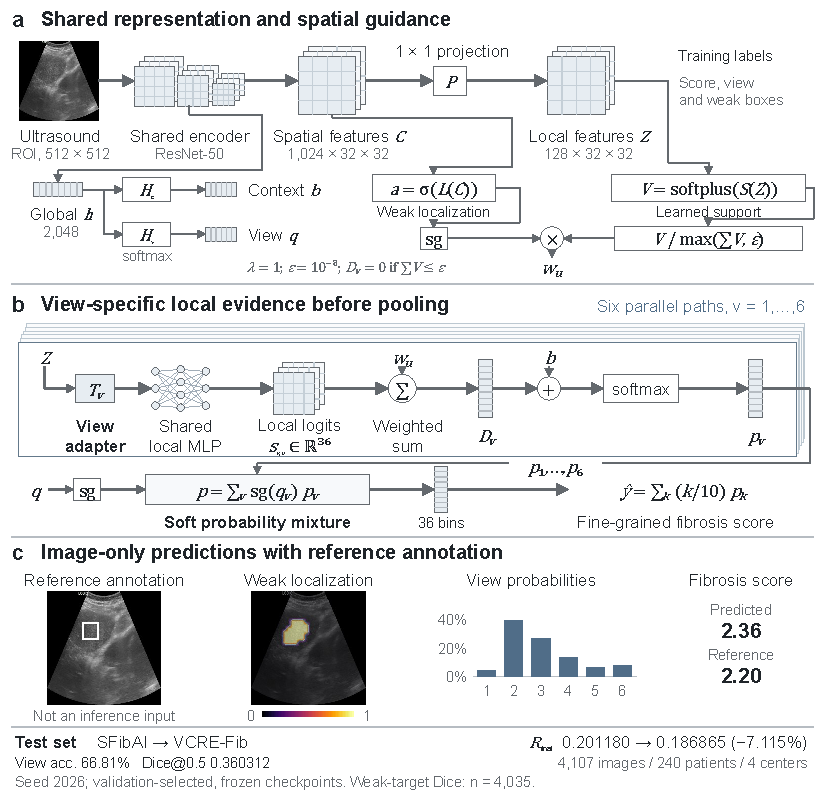
\includegraphics[width=\linewidth]{figures/assets/fig01_architecture.pdf}
\caption{\lang{\textbf{VCRE-Fib: view conditioning before spatial aggregation.} (a) A shared encoder supplies global context, view probabilities, weak localization and local features. (b) Six view-conditioned paths produce regional logit corrections, weighted by localization and learned support. Conditional distributions share context logits and are mixed by detached view probabilities. (c) One test case and test results from frozen, validation-selected checkpoints. Feature cells are schematic; $\sg$ denotes stop-gradient. Reference boxes are not inference inputs, and localization does not represent exhaustive segmentation.}{\textbf{VCRE-Fib：在空间聚合之前引入切面条件。}(a) 共享编码器提供全局上下文、切面概率、弱定位及局部特征。(b) 六条切面条件路径形成由定位与学习到的支持权重加权的区域 logit 修正。各条件分布共享上下文 logits，并依据截断梯度的切面概率融合。(c) 一个测试病例及使用经验证集选择并冻结的检查点得到的测试结果。特征格仅作示意，$\sg$ 表示停止梯度。参考框不参与推理，定位不表示完整病灶分割。}}\label{fig:architecture}
\end{figure}

\section{相关工作}\label{sec:related}
\paragraph{血吸虫病相关纤维化与超声分级。}
血吸虫感染与已经形成的器官病变需要相互补充的评估：寄生虫学、血清学及分子检测面向感染状态，影像检查则刻画肝脾异常 \citep{weerakoon2015diagnosis,sah2015imaging}。肝活检提供组织学信息，但其侵入性推动了非侵入性评估的发展；纤维化检测本身的局限也要求谨慎解释输出 \citep{bravo2001biopsy,patel2020limitations}。本文的预测目标是专家给出的超声影像评分。

对于日本血吸虫病，纤维化的解剖分布尤其重要。一项纵向队列研究发现，超声可见的肝实质纤维化与感染史相关，严重病变在治疗后的逆转有限 \citep{carlton2010morbidity}。Basel 方案在亚洲血吸虫病评估中区分门脉与间隔性纤维化形态 \citep{richter2025basel}。这些发现与影像学研究 \citep{sah2015imaging} 共同说明，在预测严重程度时保留解剖背景和可见的区域征象具有意义。

计算方法从 B-mode 纹理特征与支持向量机 \citep{yeh2003fibrosis}，发展到多参数 ultrasomics \citep{li2019ultrasomics}、面向血吸虫病的放射组学 \citep{guo2024radiomics}，以及基于 METAVIR 目标的卷积分类模型 \citep{lee2020ultrasound}。SFibAI 提供了本文沿用的细粒度评分表示 \citep{xu2026sfibai}。这些研究的采集方式、标签和队列存在差异，因此本文在相同队列划分上与 SFibAI 直接比较，并研究切面与病灶位置信息如何参与评分。

\paragraph{解剖背景与区域证据学习。}
多任务学习通过相关目标共享表征 \citep{caruana1997multitask}；SonoNet 展示了胎儿超声标准切面识别与解剖定位 \citep{baumgartner2017sononet}。区域聚合进一步将局部信息连接到图像层面的判断。Attention-based MIL 学习聚合权重 \citep{ilse2018attention}；病理影像方法通过 CLAM 的实例聚类 \citep{lu2021clam}、TransMIL 的实例关联 \citep{shao2021transmil} 以及 Additive MIL 的加性局部贡献 \citep{javed2022additive} 扩展了这一路径。FiLM 提供了条件化特征变换的通用机制 \citep{perez2018film}。VCRE-Fib 借鉴共享学习、条件化与聚合，在扫查切面背景下解释区域特征，再与全局判断融合。本文区域来自单幅超声图像，具有监督信号的切面与定位输出也实际进入评分计算。

\paragraph{弱定位与可检查的预测。}
BoxSup 与 BoxInst 使用边界框学习分割，无需逐像素掩膜 \citep{dai2015boxsup,tian2021boxinst}。本文的框标记局部异常区域，可能未包围整个病灶，因此框外响应仍是供临床复核的候选区域。概念瓶颈模型显式提供受到监督的中间概念 \citep{koh2020concept}；VCRE-Fib 提供切面和定位输出，同时保留全局路径。Grad-CAM、Grad-CAM++ 与 integrated gradients 属于事后归因方法 \citep{selvaraju2017gradcam,chattopadhay2018gradcampp,sundararajan2017axiomatic}。本文经训练获得的定位参与区域聚合，但这一作用本身不足以建立归因忠实性。显著图的 sanity checks 提示应在视觉合理性之外检验解释 \citep{adebayo2018sanity}。当前与医生标注的对照支持对空间对应关系的检查。


\section{VCRE-Fib：切面条件区域证据分级}\label{sec:method}
\subsection{任务与设计概览}
给定一幅超声 ROI 图像 $x$，模型预测严重程度分布、扫查切面与病灶弱定位图。训练数据包含评分 $y$、六类切面标签以及病灶位置标注；推理不需要切面或框标注。我们沿用 SFibAI 的离散评分点 $g_k=k/10$（$k=0,\ldots,35$），并在 0.5、1.5、2.5 处映射为四级 \citep{xu2026sfibai}。图~\ref{fig:architecture} 概括了三个步骤：学习空间线索、在切面条件下形成区域证据、将区域证据与整体判断融合。

\subsection{保留全局判断，学习可输出的空间线索}
全局路径保留整幅图像的上下文，使区域证据在整体判断基础上发挥作用。ResNet-50 编码器 \citep{he2016resnet} 产生全局特征 $h\in\mathbb{R}^{2048}$ 与 layer-3 空间特征 $C\in\mathbb{R}^{1024\times H\times W}$。对于 $512\times512$ 输入，$H=W=32$。上下文 logits 为 $b=H_c(h)\in\mathbb{R}^{36}$；切面概率为 $q=\softmax(H_v(h))\in\mathbb{R}^{6}$；弱定位图为 $a=\sigma(L(C))$。切面和定位预测既是辅助监督的学习对象，也是面向使用者的空间输出。

局部病灶框指示医生标出的相关区域，并不提供完整轮廓。弱框目标由框内响应项与框外响应占比约束组成，后者衡量框外注意力响应之和占总响应的比例；它引导空间学习，但不包含要求预测完整病灶轮廓的监督。因此，预测是否超出局部标注并对应更广泛病灶，是需要通过真实病例检查的学习结果。

\subsection{在区域聚合之前引入扫查切面}
同一局部特征需要结合其解剖背景解释。我们用 $1\times1$ 投影将空间特征变为 $Z=P(C)\in\mathbb{R}^{128\times H\times W}$。六个切面适配器 $T_v$ 分别采用 $128\rightarrow128$ 逐点卷积与 GELU，共享一个 $128\rightarrow64\rightarrow36$ MLP $f$：
\begin{equation}
s_{v,u}=f(T_v(Z)_u),\quad v=1,\ldots,6,\quad u=1,\ldots,HW .
\label{eq:local}
\end{equation}
这一操作在池化之前完成，使切面条件直接作用于各位置的评分证据。$s_{v,u}$ 表示局部 logit 贡献候选，不是单独校准的区域严重程度评分。

\subsection{以弱定位引导区域证据参与评分}
弱定位指出区域相关性，另一个支持头 $V=\operatorname{softplus}(S(Z))$ 通过分级学习聚合权重。二者共同组织区域修正：
\begin{equation}
c_{v,u}=\lambda\frac{V_u\sg(a_u)}{\max(\sum_{u'}V_{u'},\epsilon)}s_{v,u},
\qquad D_v=\sum_u c_{v,u}.
\label{eq:regional}
\end{equation}
参考配置使用 $\lambda=1$、$\epsilon=10^{-8}$；总支持不大于 $\epsilon$ 时将修正设为零。分母采用 $\sum V$，使整体偏低的定位响应能够减弱区域修正。符号 $\sg$ 表示仅在该接口截断梯度。

随后将区域修正与全局上下文结合，并通过切面概率保留条件判断的不确定性：
\begin{equation}
p_v=\softmax(b+D_v),\qquad
p=\sum_v\sg(q_v)p_v,\qquad
\hat y=\sum_k g_kp_k.
\label{eq:mixture}
\end{equation}
模型混合的是条件概率。定位图因而进入真实的区域评分路径，同时保留为可展示的输出。

\subsection{监督学习与推理输出}
按照共享表征的多任务学习方式 \citep{caruana1997multitask}，训练目标为
\begin{equation}
\mathcal L=\mathcal L_{\mathrm{grade}}(p,y)+0.1\mathcal L_{\mathrm{view}}+0.1\mathcal L_{\mathrm{box}}.
\label{eq:loss}
\end{equation}
切面采用交叉熵；弱框损失使用有效局部框，具体定义见附录~\ref{sec:appendix-implementation}。评分接口接收 $\log p$。评分损失在 $q$、$a$ 的使用接口处截断梯度，辅助损失仍更新共享编码器，评分损失仍训练上下文、局部证据与支持路径。VCRE-Fib 与 SFibAI 采用相同的混合评分损失形式及权重：两者均使用真实分值 $\hat y=0.1\sum_k kp_k$ 和 $y=0.1j$ 计算 MSE 与临床等级边界惩罚，其中 $j$ 为目标 bin。共同的评分损失公式见附录~\ref{sec:appendix-implementation}。

推理输出包括评分 $\hat y$、预测切面 $\arg\max_v q_v$ 和定位图 $a$。原图、医生标注与预测图并列呈现可供复核的空间输出。这里的输出完整性指评分之外同时保留切面和区域信息，不表示完整病灶覆盖。

\section{实验设计}\label{sec:setup}
\paragraph{数据与监督。}
本文队列由 \citet{xu2026sfibai} 所述机构超声数据库重新清洗整理而得，预测目标为既有的专家超声表现评分。我们清洗整理这些评分及既有医生病灶框，并从采集时记录的切面编号中提取六类切面标签。队列包含 35 个中心的 6,373 名患者、108,709 张 ROI 图像。训练集（train）、验证集（validation）和测试集（test）的图像数/患者数分别为 83,722/4,906、20,880/1,227、4,107/240。患者在集合之间不重叠，测试集的四个中心均在训练中出现。四模型使用相同评分数据与划分，空间监督由所保留模块决定。最高记录分数对应的框构成弱目标，并非穷尽性轮廓。全部 4,107 张测试图像均有切面标注，其中 4,035 张满足弱目标评价条件。附录~\ref{sec:appendix-cohort} 说明标注来源，表~\ref{tab:views} 列出切面名称和计数。

\paragraph{比较模型。}
本文比较 SFibAI、完整 VCRE-Fib 及两个删除变体（表~\ref{tab:matrix}）。\emph{w/o View} 保留弱定位和区域评分，移除切面头、切面专属适配器、后验混合与切面损失。\emph{w/o Weak Loc.} 保留切面条件化评分，移除定位头和弱框损失，并在式~\ref{eq:regional} 中令 $a_u=1$。两个变体均保留支持路径与全局路径，独立训练，并非从完整模型微调。这里比较的是模型设计整体，未将监督、容量和信息参与方式的影响逐一分离。
\inputtable{tab02_matrix}

\paragraph{训练、选择与冻结。}
四模型均使用相同随机种子（2026）、ResNet-50、ImageNet-1K-V2 初始化、$512\times512$ 输入、全局 batch 24、bfloat16 训练、AdamW \citep{loshchilov2019adamw}，以及相同的真实分值混合评分目标。包括完整 VCRE-Fib 在内的所有方法均以 90 epoch 为共同训练比较上限，所报告轨迹覆盖第 1--90 epoch。在验证集上从第 21--90 epoch 中依次按较低 $\risk$、较低 image COR、较早 epoch 的顺序选择检查点。共同训练设置见附录~\ref{sec:appendix-implementation}。检查点、配置和主终点在测试集比较前冻结，测试集决定观测排名。

\paragraph{评价问题。}
本文考察各空间变体是否改善基线、联合使用两类模块后分级与空间输出如何变化，以及输出呈现了哪些可检查信息。越低越好的主终点为
\begin{equation}
\risk=0.4R_{\mathrm{image}}+0.4R_{\mathrm{patient\text{-}max}}+0.2R_{\mathrm{center}} .
\label{eq:risk}
\end{equation}
各项采用锁定的临床目标风险 COR；中心项以患者数平方根加权各中心 patient-max COR，patient-median 独立报告。差异描述本次观测，未作显著性检验。表格依据未取整数值逐指标加粗最优结果，精确并列者同时加粗。

\paragraph{空间输出与可视化。}
切面报告 accuracy/macro-F1，弱目标 Dice/IoU 使用阈值 0.5。正文展示覆盖四种真实切面的四例筛选测试病例，附录另列两例验证病例。病例筛选条件、患者去重和统一显示设置见附录~\ref{sec:appendix-case-protocol}；这些病例用于说明输出信息。

\section{分级表现与空间预测结果}\label{sec:results}
\subsection{Test set 主结果}\label{sec:test}
我们首先检验，在细粒度评分中引入切面条件与局部区域信息，能否改善相同评价条件下的分级表现。在包含 4,107 张图像、240 名患者和 4 个中心的测试集上，完整 VCRE-Fib 取得最低的预设综合风险（$\risk=0.186865$），其后依次为 w/o Weak Loc.（0.191308）、w/o View（0.193799）和 SFibAI（0.201180；表~\ref{tab:main}）。三者相对 SFibAI 的绝对差分别为 $-0.014315$、$-0.009872$ 和 $-0.007380$，对应相对降低 7.115\%、4.907\% 和 3.668\%，均由未取整数值计算。该结果表明，在本次比较中，提供空间输出的三个模型均获得了相对基线的主终点收益，其中联合使用两类空间模块的完整模型表现最好。所有结果来自经验证集选择并冻结的检查点，描述当前测试集上的观测差异。
\inputtable{tab01_main}

\subsection{模块删除比较显示不同的风险改善分布}
为进一步理解上述收益，我们比较两个独立训练的删除变体。保留切面条件化的 w/o Weak Loc.\ 具有更低的 patient-max COR，而保留弱定位的 w/o View 具有更低的 image COR 和 patient-median COR（表~\ref{tab:main}）。这说明两种变体在不同评价层级上的优势并不一致。完整模型则在这些风险指标及中心平衡 COR 上均取得最低值，其综合风险比两个变体中较低的 w/o Weak Loc.\ 再降低 0.004443。因此，联合设计的收益同时体现为主终点降低和跨评价层级的风险改善。该比较反映模型设计的整体表现，尚未分离监督、容量和信息参与方式的影响，也不构成统计优越性或模块协同效应的证明。

\subsection{分级收益同时体现在图像与患者层级}
综合风险的改善伴随着具体评分指标的改善。在图像级，完整 VCRE-Fib 将 SFibAI 的 MAE 从 0.391313 降至 0.377857，四级准确率从 64.11\% 提高至 67.03\%，严重错误率从 9.98\% 降至 9.37\%（表~\ref{tab:image}）。其余图像级指标，包括 RMSE、TMAE、image COR、$\pm0.3$ 与 $\pm0.5$ 准确率及 macro-F1，也均由完整模型取得最优值。这些结果共同表明，当前观测收益覆盖连续评分误差、容差内一致性及四级判别。
\inputtable{tab05_image}

完整模型在 patient-max、patient-median 及中心平衡 COR 上仍取得最低值（表~\ref{tab:main}）。部分阈值准确率由删除变体取得更高值；完整患者级指标及这些差异见附录~\ref{sec:appendix-patient}。

\subsection{分级风险的改善伴随空间任务的取舍}
我们进一步考察，两类空间信息共同参与评分时，其辅助任务表现是否也同步提高。完整 VCRE-Fib 的切面准确率为 66.81\%、macro-F1 为 0.665861、CE 为 0.916542（4,107 张测试集图像）；弱目标 Dice/IoU 为 0.360312/0.235487（4,035 张有效图像；表~\ref{tab:auxiliary}）。相比之下，w/o Weak Loc.\ 的切面准确率和 macro-F1 更高（75.70\% 和 0.757500），w/o View 的 Dice/IoU 更高（0.430661/0.298825）。因此，最低分级风险并未伴随两项空间任务各自最优。完整模型是四者中唯一同时输出评分、切面和定位图的模型，而这一输出完整性伴随着辅助任务表现的取舍。弱目标重叠衡量与局部粗标注的一致性，不代表完整病灶分割。
\inputtable{tab07_auxiliary}

\subsection{联合输出呈现评分与空间判断的分歧}
图~\ref{fig:cases} 展示这些输出能够提供哪些具体的检查信息。四例测试集病例覆盖四种真实切面，每行并列呈现原始超声、医生标注与定位预测，并保留参考/预测评分及完整切面名称。(a)--(c) 展示定位响应与标注的对应；其中 (a) 的评分接近参考值（2.4/2.409），切面却将真实左肋下横切面误判为剑突下矢状切面。该例表明，评分接近并不保证空间判断正确，而联合输出使这类分歧能够被直接查看。

(d) 的参考/预测评分为 1.4/1.491，在固定色标和阈值下呈现超出局部矩形框的响应，附录另列两例验证集示例。框外响应提供了可检查的位置，但既可能对应相关组织，也可能是错误激活，不能据此确认完整病灶覆盖或临床正确性。所有定性病例均由用于定量评价的冻结检查点生成；其作用是展示可检查的信息，不附加医生解释，也不据此主张已验证的临床复核收益。
\begin{figure}[!tb]
\centering
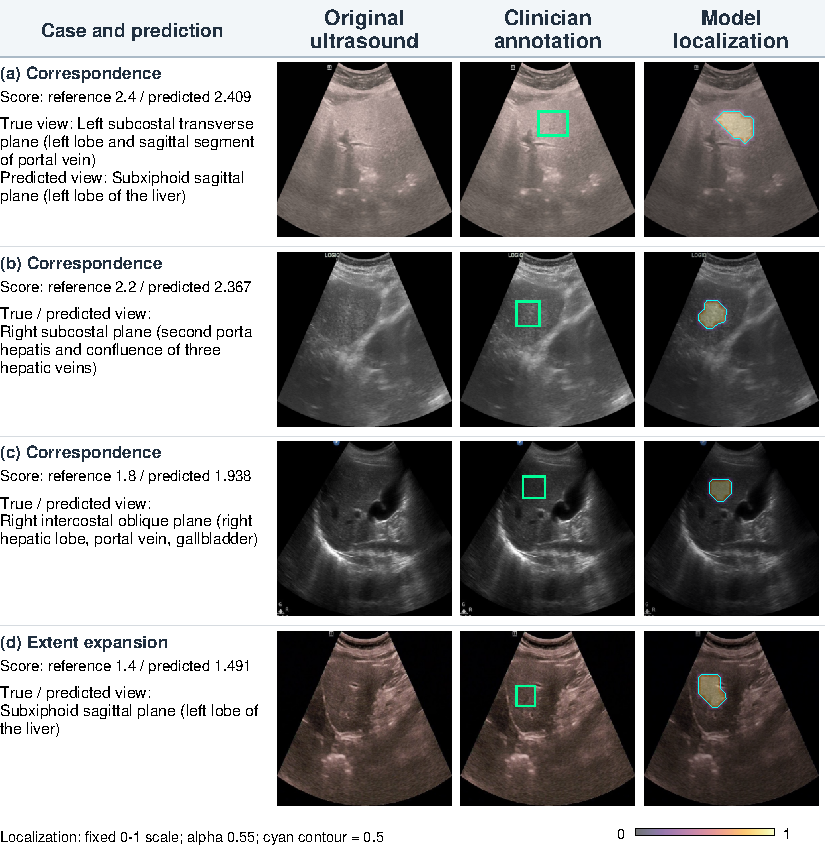
\includegraphics[width=\linewidth]{figures/assets/fig06_cases.pdf}
\caption{\lang{Four selected test cases, with reference and predicted scores and acquisition views at left. Predictions use the frozen checkpoint evaluated quantitatively. Rows (a)--(c) show localization correspondence; (d) shows a response beyond local boxes. Green boxes denote clinician annotations; localization uses a $[0,1]$ scale, opacity 0.55, and a cyan 0.5 contour. In row (a), the predicted view differs from the reference. These selected examples illustrate spatial outputs without establishing population localization performance or complete lesion extent.}{四个筛选的测试集病例，左侧标出参考及预测评分和扫查切面。预测使用参与定量评价的冻结检查点。(a)--(c) 展示定位对应，(d) 展示局部框外响应。绿色框为医生标注；定位色标为 $[0,1]$、透明度为 0.55，青色轮廓阈值为 0.5。(a) 的预测切面与参考切面不同。这些筛选示例用于展示空间输出，不代表总体定位水平或完整病灶范围。}}
\label{fig:cases}
\end{figure}


\subsection{联合预测的计算开销}
我们进一步量化同时提供评分与两类空间输出的计算代价。在同一 A100-SXM4-80GB 上按 FP32 测量，SFibAI、w/o View、w/o Weak Loc.\ 和完整 VCRE-Fib 的 batch-one 中位延迟分别为 5.620、6.171、7.122 和 7.371 ms。完整模型相对 SFibAI 增加 7.81\% 参数、4.24\% 计数 MACs，以及 1.751 ms 中位延迟。附录表~\ref{tab:resources} 同时报告 batch 1 和 8 的延迟、P95 与显存，给出分级和输出收益所对应的资源开销。

\section{讨论}\label{sec:discussion}
分级风险、切面准确率和弱目标重叠分别评价严重程度预测、采集切面识别及与局部标注的一致程度。完整模型取得最低分级风险，而删除变体具有更高的空间任务指标，说明评价时应同时考察评分及各项伴随输出。模块删除比较评价的是整体设计，未分离监督、模型容量和信息使用方式的影响，任务取舍背后的机制仍待明确。

局部矩形框为空间学习提供位置线索。将区域响应图与原始图像及医生标注框对照，可以直接检查响应与这些线索的对应关系，并发现可供进一步查看的区域。弱目标重叠衡量位置一致性，完整病灶覆盖则是另一项评价目标。框外响应可能对应相关组织或错误激活，更完整的空间参考与医生复核有助于区分这些情况。

对于临床复核，联合输出提供三个检查对象：预测切面、区域响应和最终评分。所示病例中评分接近但切面预测错误的情况，展示了这些输出如何呈现同一预测的不同方面。将它们与原始图像并列呈现，可以分别检查解剖背景和局部响应。其实际获益仍有待通过阅片者研究评价，具体包括错误识别、判断修订的恰当性和复核时间。

部署研究应在本文报告的模型开销之外，于目标硬件上联合测量预处理、推理和结果展示。独立队列评价应检验不同患者人群与采集条件下的分级及空间输出表现。

\section{结论}\label{sec:conclusion}
VCRE-Fib 将切面条件化的区域证据与全局预测结合，用于日本血吸虫病相关肝纤维化的超声精细分级。在使用冻结检查点的比较中，完整模型的测试集综合风险较 SFibAI 降低 7.115\%，同时输出评分、切面和区域信息。完整模型取得分级收益的同时，对应删除变体在切面准确率或弱目标重叠上表现更高。这种任务取舍说明，评价联合预测系统时，除最终分级表现外，还应分别考察各项空间输出的质量。联合输出使解剖及区域判断能够与评分一同接受检查。后续评价应考察这些输出辅助医生复核的实际作用，以及它们在独立队列中的表现。

\label{main-text-end}
\clearpage
\section*{伦理声明}\label{post-main-start}
本研究对超声图像及相关标注的回顾性使用已获得相应机构伦理批准。所有参与者均在入组前签署书面知情同意。
\section*{可复现性声明}
第~\ref{sec:method}--\ref{sec:setup} 节给出模型结构与评价协议。附录~\ref{sec:appendix-implementation} 说明数据整理和共同训练设置，附录~\ref{sec:appendix-results} 报告完整测试集指标及资源测量，附录~\ref{sec:appendix-analyses} 说明病例选择与显示规则，附录~\ref{sec:appendix-selection} 提供检查点选择及四模型训练轨迹。
\section*{AI 使用声明}
OpenAI Codex 协助检查实现、起草、翻译和修改论文、核对参考文献、编译文档，以及呈现既有结果与病例图，未生成实验观测。作者对科学内容及其解释负责。
\bibliographystyle{iclr2027_conference}
\bibliography{references}
\section*{附录}
\addcontentsline{toc}{section}{附录}
\label{appendix-start}
\appendix
\setcounter{table}{0}
\setcounter{figure}{0}
\setcounter{equation}{0}
\renewcommand{\thetable}{S\arabic{table}}
\renewcommand{\thefigure}{S\arabic{figure}}
\renewcommand{\theequation}{S\arabic{equation}}
\renewcommand{\theHtable}{appendix.\arabic{table}}
\renewcommand{\theHfigure}{appendix.\arabic{figure}}
\renewcommand{\theHequation}{appendix.\arabic{equation}}

\section{队列、标注与实现细节}\label{sec:appendix-implementation}
\subsection{队列来源与标注范围}\label{sec:appendix-cohort}
\paragraph{参考评分与队列整理。}
本文队列由 \citet{xu2026sfibai} 所述机构超声数据库重新清洗整理而得，沿用专家给出的超声表现评分，范围为 0.0--3.5，间隔为 0.1。原研究的标注方案将四个临床等级细化为这一评分尺度，并说明了统一培训、集中复核和对评分分歧进行专家复核的流程。本研究对既有图像与标注进行清洗和整理，未重新评定评分。本文队列及划分与原研究不同，SFibAI 基线在本文划分上训练和评价。

\paragraph{扫查切面与病灶位置标注。}
六类切面标签从图像采集时记录的切面编号中提取，并在数据清洗时整理。病灶位置监督同样沿用 \citet{xu2026sfibai} 所述的既有医生矩形框，经清洗整理后使用。这些框标出图像中需要关注的区域，并附有原始分级标注。因此，切面标签描述采集时记录的扫查切面，矩形框则指示图像内部的局部区域。推理时无需提供这两类标注。

\paragraph{覆盖范围与弱目标。}
整理后的记录为每张图像保留切面及病灶位置标注，但并非每条记录都提供符合条件的非空弱目标。框监督使用目标分数为正的有效非空框，详见附录~\ref{sec:appendix-implementation}。弱定位评价包含 4,035 张有效测试图像，切面评价包含全部 4,107 张测试图像。局部框并未勾画完整病灶轮廓，因此框外响应的空间相关性仍需单独评价。

\inputtable{tab12_cohort}
\subsection{SFibAI 基线与训练实现}
\paragraph{明确 SFibAI 基线身份。}
方法来源为 \citet{xu2026sfibai}。基线采用作者的公开实现。基线使用 ResNet-50、全局平均池化、线性 $2048\rightarrow36$ 头、softmax 与 0.0--3.5 上的期望分数，没有切面和定位预测头。上游允许指定初始化检查点，未提供时使用随机初始化骨干；共同 ImageNet 初始化是针对本次比较的适配，不是上游默认值。

\paragraph{评分目标。}
VCRE-Fib 与 SFibAI 采用相同的纤维化评分尺度和混合损失权重 $(\alpha,\beta,\gamma)=(1,0.02,0.02)$。对于目标 bin $j\in\{0,\ldots,35\}$ 和预测概率 $p_k$，两者均先将 bin 索引转换为真实临床分值，再计算 MSE 与临床等级边界惩罚：
\[
\begin{aligned}
y&=0.1j,\qquad \hat y=0.1\sum_{k=0}^{35}kp_k,\\
L_{\mathrm{grade}}&=L_{\mathrm{KL,local}}+0.02(\hat y-y)^2
 +0.02|\hat y-y|\mathbf{1}(\hat c\ne c).
\end{aligned}
\]
其中 $c$、$\hat c$ 分别由 $y$、$\hat y$ 按 0.5、1.5、2.5 阈值映射为四级，分数恰好等于阈值时归入较高等级。上式为逐图损失，各项在 batch 内取均值。MSE 和绝对误差边界项均在 0.0--3.5 的真实分值尺度上计算。

局部 KL 采用定义在全部 36 个 bin 上、标准差为一个 bin 的归一化高斯软目标，并在以目标 bin 为中心的局部窗口内计算。两方法采用这一混合评分损失形式，评分单位及各分项权重保持一致。

\paragraph{训练协议。}
四模型均采用相同随机种子（2026）、ImageNet-1K-V2 权重、batch size 24、bfloat16、AdamW 学习率与权重衰减均为 $10^{-4}$，以及每 15 epoch 将学习率乘以 0.6 的 StepLR。ROI 预处理、拉伸缩放、直角旋转/饱和度增强、患者互斥划分及上述评分目标相同。这统一了公开 SFibAI 中不同的裁剪、增强和初始化默认值。SFibAI、两个删除变体和完整 VCRE-Fib 的训练轨迹及检查点比较均使用相同的 90 epoch 上限。在验证集上从第 21--90 epoch 中依次按较低 $\risk$、较低 image COR、较早 epoch 的顺序选择检查点，替换上游容差准确率选择器。四者所选 epoch 依次为 65、80、39、47。本比较使用重新整理的队列，不声称复现 SFibAI 原始队列实验。

\paragraph{VCRE-Fib 的新增监督。}
六分类切面交叉熵权重为 0.1。弱框损失结合框内 log-sum-exp 池化（温度 10）和框外响应占比，内部权重为 1，总权重为 0.1。仅有效、非空且目标 bin $j>0$ 的弱框参与；排除精确分数 0.0，不排除整个 F0。弱目标在 ROI 坐标系中变换，支持图通过评分学习。辅助损失更新共享编码器，仅在评分接口截断 $q$ 与 $a$。w/o View 删除切面头、六个适配器、后验混合和切面 CE，保留无切面条件的区域证据与弱定位。w/o Weak Loc.\ 删除定位头和弱框损失，使用中性 $a_u=1$ 并保留切面与支持路径。两个删除变体均由规定初始化独立训练。


\FloatBarrier
\section{完整测试结果与资源测量}\label{sec:appendix-results}
\subsection{Test set 主结果}
冻结的验证集选择的检查点在 4,107 图、240 患者、4 中心上评价。排序为 VCRE-Fib、w/o Weak Loc.、w/o View、SFibAI（表~\ref{tab:comparison}），$\risk$ 越低越好。正文表~\mainref{tab:main}--\mainref{tab:auxiliary} 报告主终点、图像与空间结果；患者级详细指标见附录~\ref{sec:appendix-patient}。
\inputtable{tab04_comparison}

\paragraph{指标定义。}
令 $e=|\hat y-y|$，$d$ 为阈值 0.5、1.5、2.5 对应的四级等级绝对差。锁定的单项风险为
\[
\operatorname{COR}=0.35e/3.5+0.15\mathbf{1}(e>0.3)+0.15\mathbf{1}(e>0.5)+0.25d/3+0.10\mathbf{1}(d\ge2).
\]
Patient-max 和 patient-median 两种方法均对参考评分与预测评分分别进行患者内聚合。中心平衡 COR 按患者数平方根加权。TMAE 为 $\operatorname{mean}\max(e-0.5,0)$，严重错误率为 $\operatorname{mean}\mathbf{1}(e>1.0)$，与 COR 中的跨两级错误不同。
\subsection{患者级分级详细结果}\label{sec:appendix-patient}
将图像评分分别按 patient-max 和 patient-median 聚合后，完整模型仍具有最低的 COR（分别为 0.200528 和 0.154344），同时取得最低的 median MAE（0.339273；表~\ref{tab:patient}）和中心平衡 COR（0.177453；正文表~\mainref{tab:main}）。这一结果使主终点收益得到不同聚合方式下的风险指标支持。不过，风险降低并不意味着每个阈值指标均最优：w/o Weak Loc.\ 的 patient-max $\pm0.5$ 准确率更高（67.50\%），w/o View 的 median 四级准确率更高（72.08\%）。完整模型的优势因此主要表现为整体风险及多项评分指标的共同改善。
\inputtable{tab06_patient}

\subsection{补充分级指标与中心结果}
各中心估计是描述性的，其中一个中心仅有两名患者。测试集与验证集导出保留逐级支持数、召回率和 COR 各分项。四级概率由 36 个 bin 按等级求和；图像 AUPRC 使用 average precision，ECE 使用十个分箱。缺少正例或负例时，逐类 AUROC/AUPRC 记 N/A；不作患者概率聚合。
\inputtable{tab14_additional}
\inputtable{tab15_centers}
\FloatBarrier

\subsection{资源测量}
\label{sec:appendix-resources}
\inputtable{tab09_resources}
四个冻结模型均在同一 NVIDIA A100-SXM4-80GB 上测量，使用 PyTorch 2.11.0+cu128、FP32、关闭 TF32、$512\times512$ 输入。预热 50 次后进行 200 次同步墙钟计时。延迟按批次报告，输入已在 GPU 上，只计模型前向，不含加载与传输。峰值已分配显存以 MiB 表示。计算量只统计实际执行的 Conv2d/Linear，不含逐元素运算、池化与归一化；所报 FLOPs 为计数 MACs 的两倍。

\FloatBarrier
\section{空间预测与定性示例}\label{sec:appendix-analyses}
\subsection{切面名称与弱目标统计}
\inputtable{tab13_views}


\paragraph{补充弱目标统计。}
完整 VCRE-Fib 在测试集上的框内平均响应、框外响应占比、框内/框外平均响应比分别为 0.570815、0.666595、359,012.493654；w/o View 对应为 0.499237、0.550558、1,678,411.504391。框外响应占比为目标框外注意力响应之和占总响应的比例。最后一项的分母截断于 $10^{-8}$，全视野框可产生很大比值。这些是描述性响应统计，并非定位准确性指标。表~\ref{tab:views} 比较两个含切面头模型的逐类召回率，评价产物另提供预测频率与混淆矩阵。

\subsection{病例选择与显示协议}\label{sec:appendix-case-protocol}
切面报告 accuracy/macro-F1，弱目标 Dice/IoU 使用阈值 0.5。从包含 12 个测试病例和 4 个验证病例的候选池中，选取覆盖四种真实切面的 4 个完整模型测试病例用于正文，另选两例验证病例用于附录。定位对应候选在切面内优先按弱框 Dice 选择。范围扩展候选要求框外响应占比 0.5--0.9、Dice 大于 0.1、阈值响应与框内相交，且至少 10\% 响应面积在全部显示框之外。各池内部按患者去重。三列使用相同处理后 ROI、固定 $[0,1]$ 定位色标、0.55 透明度和青色 0.5 轮廓。这些是筛选示例，当前不附加扩展区域的医生解释。

正文展示四个筛选的测试集病例。图~\ref{fig:valcases} 展示两例定位响应超出局部框的验证集病例，独立于测试集排名与空间指标；其中首例的预测切面与参考切面不同。
\begin{figure}[!htbp]
\centering
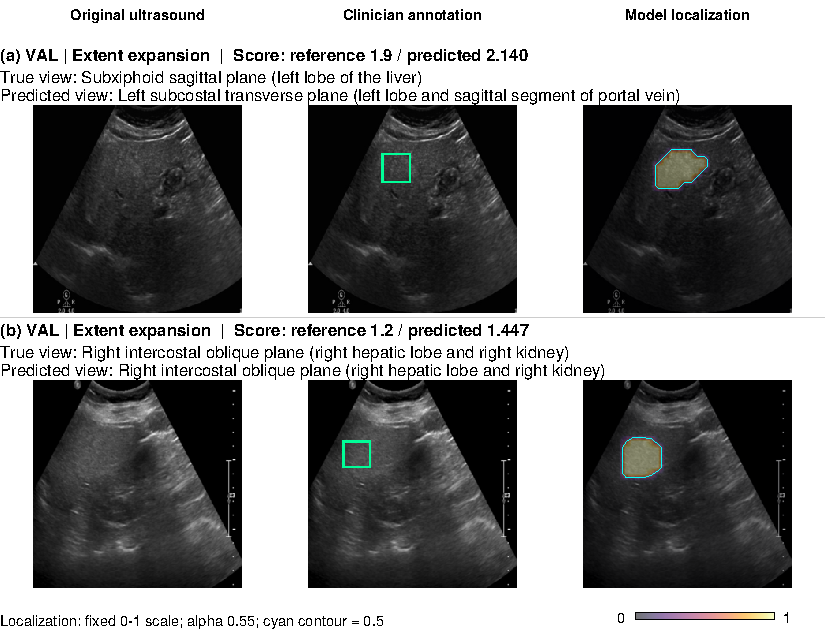
\includegraphics[width=\linewidth]{figures/assets/fig06_validation_cases.pdf}
\caption{定位响应超出局部框的验证集病例。预测使用参与定量评价的冻结检查点。三列依次呈现原始 ROI、医生标注与模型定位，文字标出参考及预测评分和扫查切面。首例的预测切面与参考切面不同。框外响应指出可供检查的位置，不表示已确定完整病灶范围。}
\label{fig:valcases}
\end{figure}

\FloatBarrier
\section{验证集检查点选择与训练诊断}\label{sec:appendix-selection}
对于 SFibAI、w/o View、w/o Weak Loc.\ 和完整 VCRE-Fib，验证集所选 epoch 分别为 65、80、39、47，$\risk$ 为 0.172661、0.157844、0.159315、0.156067。验证集含 20,880 张图像、1,227 名患者和 33 个中心。附录表~\ref{tab:freeze} 记录四个冻结检查点，图~\ref{fig:training} 展示相同 90 epoch 上限下的四条训练轨迹。这些记录交代检查点选择来源，模型的观测排序仍由测试集主终点确定。
\inputtable{tab10_freeze}
四模型均用四 GPU、SyncBatchNorm 和全局 batch 24，共同训练设置见附录~\ref{sec:appendix-implementation}。在验证集上从第 21--90 epoch 中依次按较低 $\risk$、较低 image COR、较早 epoch 的顺序选择检查点，并在测试集评价前冻结。图~\ref{fig:training} 展示全部 90 个逐轮记录，未作平滑。各模型总损失包含不同的辅助项，用于模型内部训练诊断。图~\ref{fig:losses} 展示完整模型的损失分项。
\begin{figure}[!htbp]
\centering
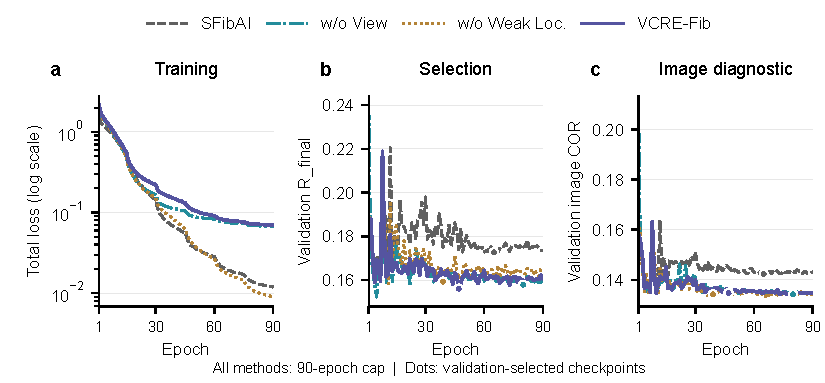
\includegraphics[width=\linewidth]{figures/assets/training_curves.pdf}
\caption{\lang{Training and validation trajectories under a common 90-epoch cap. (a) Total training loss on a logarithmic axis, including each model's auxiliary terms. (b) Validation $R_{\mathrm{final}}$. (c) Validation image COR. Curves show unsmoothed epoch-level observations; dots mark the validation-selected checkpoints in Table~\ref{tab:freeze}.}{统一 90 epoch 上限下的训练与验证集轨迹。(a) 含各模型辅助项的训练总损失，纵轴为对数尺度。(b) 验证集 $R_{\mathrm{final}}$。(c) 验证集 image COR。曲线为未经平滑的逐轮观测，圆点标记表~\ref{tab:freeze} 中由验证集选择的检查点。}}\label{fig:training}
\end{figure}

\begin{figure}[!htbp]
\centering
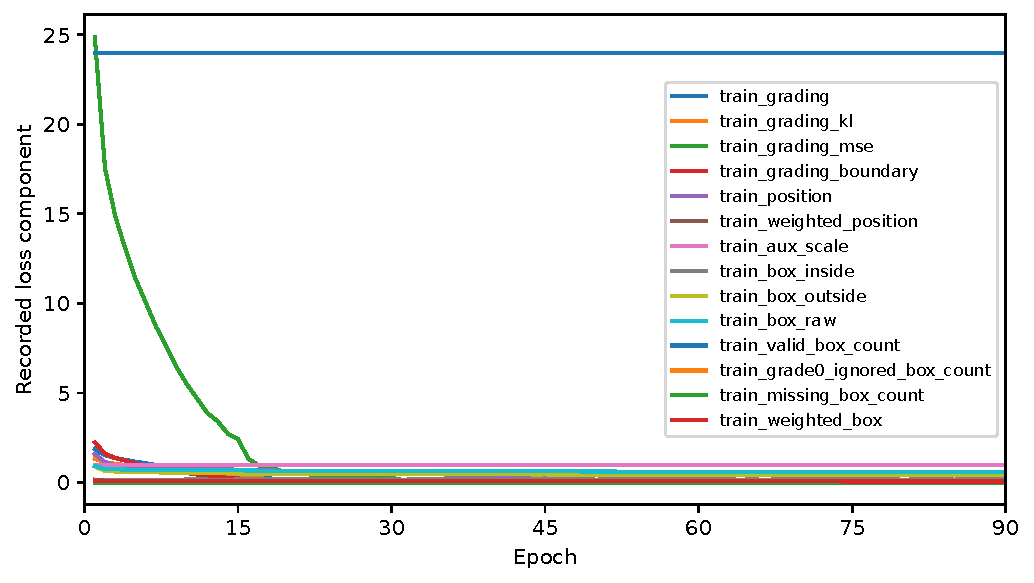
\includegraphics[width=\linewidth]{figures/assets/synap_loss_components.pdf}
\caption{\lang{Full VCRE-Fib loss components under the same 90-epoch cap, shown as training diagnostics rather than estimates of module effects.}{完整 VCRE-Fib 在相同 90 epoch 上限下的训练损失分项，用于训练诊断，不作为模块效应估计。}}\label{fig:losses}
\end{figure}

\FloatBarrier


\end{document}
